\bookchapter{第三十七章：正規化革命——從“寫程式碼”到“指揮AI寫程式碼”}

\chapterintro{恭喜你，翻開這本書的你，正站在一場職業正規化革命的正中央。這場革命的起點，是 2025 年一個程式設計師在社交媒體上發的一句話。聽起來有點戲劇性？但事實就是這樣。}

\booksection{一、Vibe Coding 的誕生：一句話引發的運動}

2025 年 2 月，Andrej Karpathy——這個名字請先記住，後面還會見到他好幾次——在社交媒體上發了一條後來被反覆引用的推文：“有一種新程式設計方式叫 Vibe Coding，你完全憑感覺（vibes）來，忽略程式碼細節，讓 AI 包攬一切。你看到什麼就說什麼，複製貼上，基本上能用就行。”

這條看起來隨口一說的發言，其實精準命名了一場已經悄然發生的正規化轉移：人類不再逐行編寫程式碼，而是用自然語言描述意圖，由 AI 完成實現。Karpathy 的措辭帶著一絲戲謔，但背後是個深刻的洞察：當 AI 的程式碼生成能力跨過某個閾值之後，程式設計的瓶頸就不再是“這行程式碼我能不能寫出來”，而是“這件事我到底想不想得清楚”。

\begin{tcbinfo}{小貼士：Vibe 是什麼？}
Vibe 直譯是“氛圍、感覺”。Vibe Coding 就是“跟著感覺指揮 AI 程式設計”——你描述想要什麼，AI 負責實現。記住這個詞，它是這場革命的“出生證明”。

\end{tcbinfo}

從那一刻起，“編碼”這個詞的含義開始分裂：傳統的編碼是把設計翻譯成語法；新的編碼是把意圖翻譯成指令。前者考驗手指，後者考驗腦子。

Vibe Coding 這個詞很快從戲謔變成了嚴肅的工程概念。到 2026 年中期，它已經從一個社交媒體上的梗，演化為一套完整的方法論體系——涵蓋需求表達、上下文管理、迭代驗證到品質保障的全流程。人們也意識到：“憑感覺”只是入門階段的狀態，真正高效的 AI 程式設計需要一套系統化的思維方式。而這套思維方式，就是本書要給你的東西。

\booksection{二、2026 年現狀：Agentic Engineering 時代}

到了 2026 年 8 月，AI 程式設計領域已經經歷了幾次重要的正規化迭代。Vibe Coding 是最初的火花，但很快大家發現：光“憑感覺”和 AI 聊天，產出的程式碼品質極不穩定——有時驚豔，有時翻車。於是正規化開始進化：從簡單的對話式程式設計，走向結構化的 Agent 工程。

又是 Karpathy，2026 年初提出了 Agentic Engineering 的概念。與 Vibe Coding 的“說了就生成”不同，Agentic Engineering 強調：給 AI 一個目標，讓它自主規劃步驟、呼叫工具、驗證結果、迭代修正。AI 不再只是一個程式碼生成器，而是一個能感知環境、做出決策、執行動作的智慧體（Agent）。

這個轉變帶來了三個關鍵變化：

\begin{enumerate}
  \item 互動模式變了：從"一問一答"變成"設定目標後放權"。
  \item 工作產物變了：從"一段程式碼"變成"一個完整的專案"。
  \item 人的角色變了：從"逐行稽核程式碼"變成"定義邊界、驗收結果"。
\end{enumerate}

數字不會說謊：Cursor 在 2026 年 4 月釋出的 Cursor 3 版本中，Agent 模式的使用率首次反超 Tab 補全模式，標誌著開發者已經大規模轉向這種工作方式；而 Claude Code 這個終端原生的 AI 程式設計工具，到 2026 年中期已達到年化收入 25 億美元的規模。下面的趨勢圖能讓你直觀感受這個交叉時刻：

\begin{center}
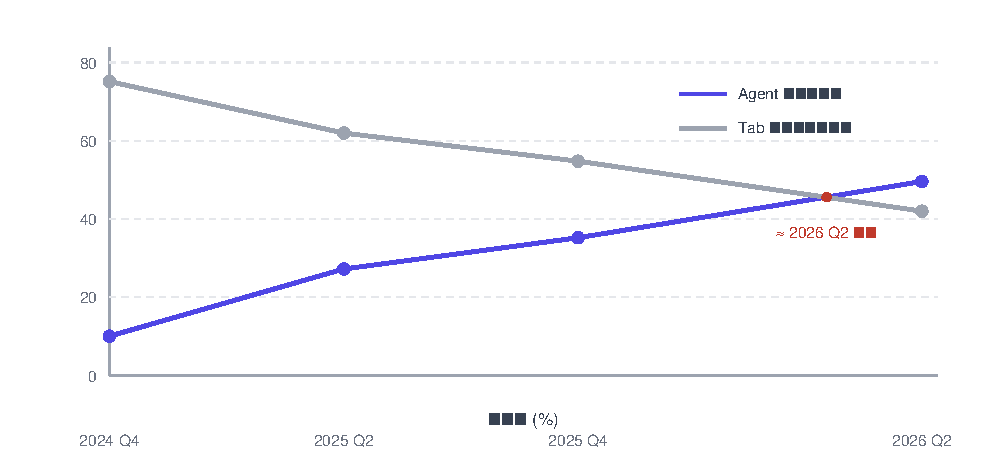
\includegraphics[width=0.92\linewidth]{figures/fig-di-san-shi-qi-zhang-1}
\\[2pt]\small 圖 1：AI 程式設計互動模式使用率變化趨勢（基於行業調研資料估算，2026 Q2 Agent 模式反超 Tab 補全）
\end{center}

但說句實在話：工具和模型的變化只是表象。無論你用 Cursor 還是 Claude Code，無論底層模型是 GPT-5 還是 Claude 4.5，成功的 AI 程式設計實踐者都在遵循同一套底層方法論。這就是本指南要教給你的東西。

\booksection{三、核心認知轉變：從 Coder 到 Conductor}

傳統程式設計教育教你如何成為一個 Coder——理解語法、記憶 API、除錯邏輯錯誤。AI 程式設計時代，這個角色正在被重新定義。你不再需要親手把每一行程式碼寫出來，但你需要成為一個“指揮官”（Conductor）：定義戰場、制定規則、分配任務、驗收成果。

這個轉變的核心不在於“你會不會寫程式碼”，而在於“你會不會想清楚要做什麼”。一個優秀的指揮官不一定是最好計程車兵，但他必須最清楚戰役的目標、地形和兵力部署。同理，一個優秀的 AI 程式設計實踐者不一定精通每一種程式語言的語法細節，但他必須最清楚專案的目標、架構約束和品質標準。

這張表值得你多看兩遍——它概括了這次角色轉變的全部內涵：

\begin{center}
\begin{tabularx}{\linewidth}{|X|X|X|}
\hline
\textbf{維度} & \textbf{傳統 Coder} & \textbf{AI 指揮官（Conductor）} \tabularnewline
\hline
核心技能 & 語法記憶、API 呼叫、除錯 & 需求定義、上下文管理、驗收判斷 \tabularnewline
工作方式 & 逐行編寫程式碼 & 描述意圖，審查產出 \tabularnewline
品質把控 & 自己寫的，自己心裡有數 & 透過測試和審查驗證 AI 產出 \tabularnewline
知識要求 & 深度掌握特定語言/框架 & 廣度理解技術全貌，深度理解業務邏輯 \tabularnewline
瓶頸所在 & 編碼速度和語法記憶 & 思考清晰度和表達能力 \tabularnewline
錯誤來源 & 語法錯誤、邏輯遺漏 & 需求模糊、上下文不足 \tabularnewline
\hline
\end{tabularx}
\end{center}

\begin{center}\small\color{gray}傳統 Coder 與 AI 指揮官的能力維度對比\end{center}

這絕不是說程式設計知識不重要了。恰恰相反：當你能看懂 AI 寫的程式碼時，你才能有效地審查和修正它；當你理解資料結構和演演算法時，你才能判斷 AI 的方案是否合理。知識儲備決定了你的“指揮上限”——但知識的角色從“執行工具”變成了“判斷依據”。

\booksection{四、為什麼方法論比工具更重要}

工具每三個月迭代一次，方法論每三年才進化一次。學會一個工具的操作，三個月後可能就過時了；掌握一套思維方式，三年後依然適用。

很多人在入門 AI 程式設計時，第一件事就是追問“哪個工具最好”“哪個模型最強”。這些問題不是不重要，但它們問錯了優先順序。2026 年 8 月的工具格局和 2025 年 8 月已經完全不同——Trae、Qoder 等工具興衰起伏，Cursor 從外掛變成了獨立 IDE 又進化到 Cursor 3，Claude Code 從實驗性專案變成了終端程式設計的主流選擇。但在這劇烈變化背後，成功實踐者遵循的思維原則幾乎沒有改變。

這就是為什麼本書不會把篇幅花在教你某個工具的具體操作上——那些內容寫完就會過時。相反，本書的全部重心放在一套經過驗證的思維方法論上：如何思考需求、如何與 AI 溝通、如何驗證產出、如何持續迭代。掌握了這套方法論，你換任何工具都能快速上手；只學了工具操作，換一個工具就要從零開始。

\begin{tcbinfo}{給零基礎讀者的定心丸}
如果你是零基礎，別被“方法論”三個字嚇到。方法論不是抽象的哲學，它就是一套“遇到問題該怎麼想”的操作手冊。就像學做菜：你可以照著菜譜一步步來（工具操作），但真正的大廚理解的是“為什麼要這樣調味”“火候怎麼控制”（方法論）。本書會從最基礎的概念講起，每個原則都配具體的對比案例，確保你不僅理解“是什麼”，更能掌握“怎麼做”。

\end{tcbinfo}

\begin{tcbpractice}{來動手：給現在的你拍張"角色照"}
拿出一張紙，寫下三個問題的答案：(1) 你現在是怎麼用 AI 幫你寫程式碼的（如果用過的話）？(2) 你更像上表中的“Coder”還是“指揮官”？(3) 你希望三個月後的自己會怎樣描述自己的工作方式？寫完後夾在書裡，讀完第四十七章再回來看——你會發現變化比想象中快。

\end{tcbpractice}

\begin{tcbsummary}{本章小結}
\begin{itemize}
  \item 2025 年 Karpathy 用"Vibe Coding"命名了 AI 程式設計革命：從逐行寫程式碼，變成用自然語言描述意圖
  \item 2026 年進化到 Agentic Engineering：給目標、放權、AI 自主規劃執行，人負責驗收
  \item Cursor 3 的 Agent 模式使用率首次反超 Tab 補全；Claude Code 年化收入達 25 億美元
  \item 你的新角色是 Conductor（指揮官）：定義戰場、制定規則、分配任務、驗收成果
  \item 工具每三個月迭代一次，方法論每三年才進化一次——學方法論，不學操作
\end{itemize}

\end{tcbsummary}
